\chapter{Architektur}
\label{architektur}

Das Gesamtsystem setzt sich aus insgesamt vier Komponenten zusammen: die Datenbank, der Webserver, die Fehlerquelle und das Zielsystem von OpenStreetMap. 
Die einzelnen Komponenten sind über \gls{REST}-Schnittstellen miteinander verbunden. 
Dabei sind das Zielsystem (OpenStreetMap) und die Fehlerquelle (Keepright, siehe Kapitel \ref{datenquellen}) Fremdsysteme, bei welchen die Schnittstellen gegeben waren. 
Unsere eigenen Server haben wir entsprechend angepasst und auch via REST zugänglich gemacht.

\begin{figure}[H]
	\centering
	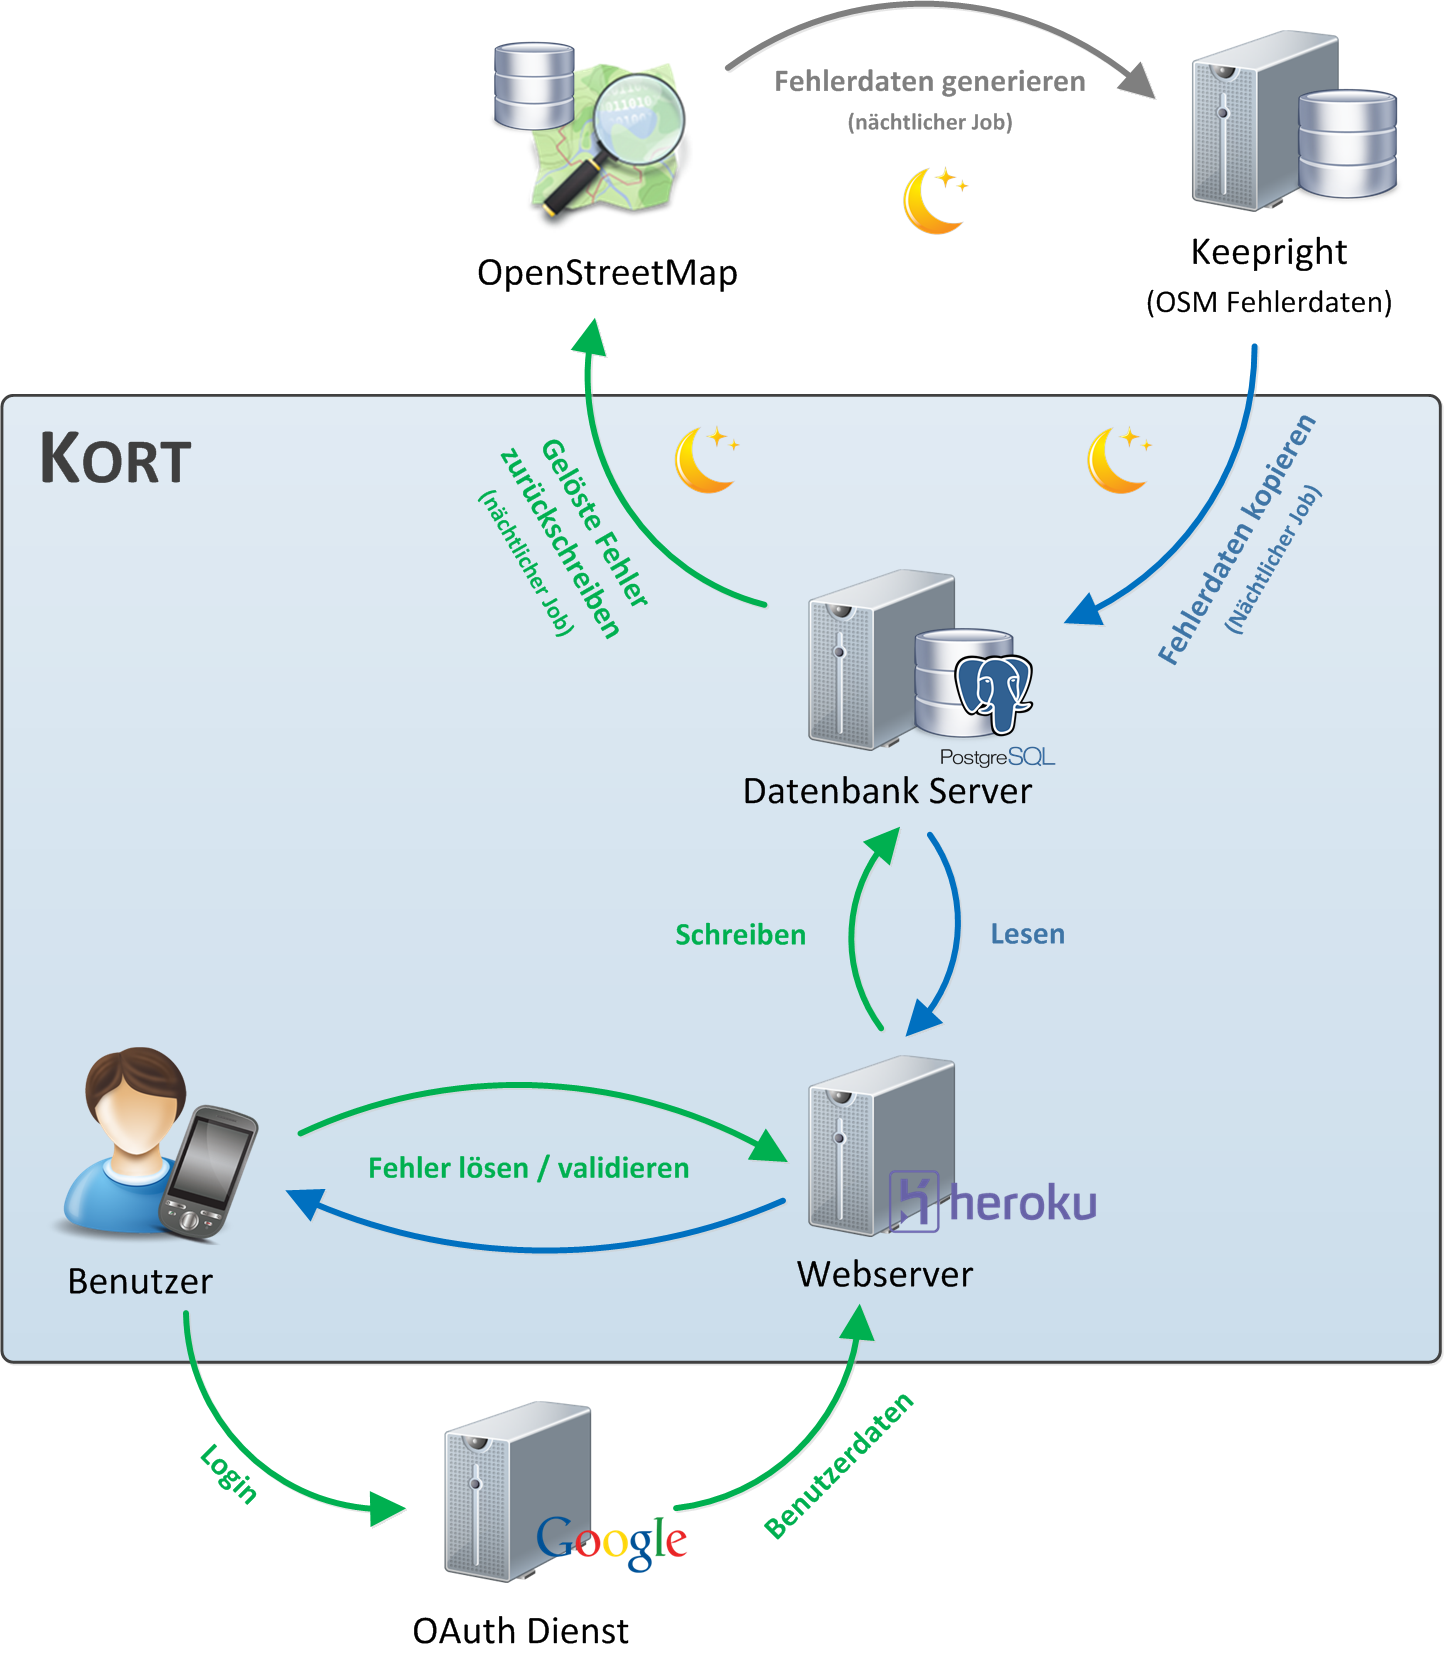
\includegraphics[scale=0.32]{images/implementation/backend/kort-big_picture}
	\caption{Übersicht des Gesamtsystems}
	\label{image-kort-big-picture}
\end{figure}

Das Backend besteht aus zwei logisch und derzeit auch physisch getrennten Servern. 
Der Webserver liefert die \gls{WebApp} aus und ist auch der einzige Kommunikationspartner für das Frontend. Dies ist zum einen eine architektonische, zum anderen eine technische Entscheidung.

\begin{itemize}
\item Das Frontend muss sich nicht darum kümmern woher es welchen Dienst bezieht
\item Die Same-Origin-Policy\cite{sop} einiger Server lässt keine direkte Kommunikation zwischen \emph{fremdem} JavaScript und dem Server zu
\end{itemize}

Der Webserver ist somit der Dreh- und Angelpunkt der Applikation, jegliche Informationen von und zum Frontend durchläuft diese zentrale Komponente.

\begin{figure}[H]
	\centering
	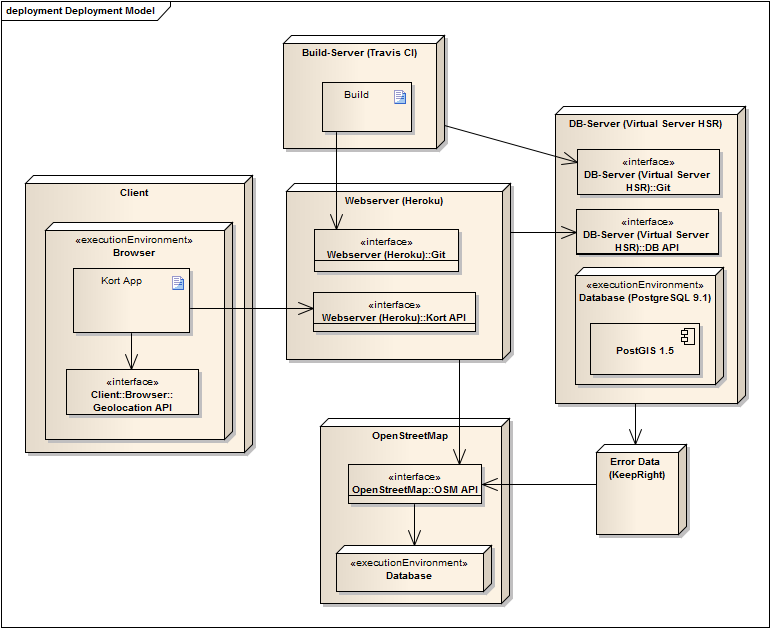
\includegraphics[width=\textwidth]{images/uml/deployment_diagram}
	\caption{Deployment-Diagramm}
	\label{deplyoyment-diagram}
\end{figure}

\section{Umsysteme}
\todo[inline]{Umsysteme (OSM, Keepright) beschreiben. Hinweis OSM-Stammtisch}

\section{Authentifizierung}
\todo[inline]{Warum OAuth?}

\section{Verteilung der Server}
\todo[inline]{Verteilung der Server beschreiben}

\section{REST}
\todo[inline]{Warum wurde REST verwendet?}

\section{Datenbank}
\todo[inline]{Konzept der Datenbank (Views, Schemas)}